% Prof. Dr. Ausberto S. Castro Vera
% UENF - CCT - LCMAT - Curso de Ci\^{e}ncia da Computa\c{c}\~{a}o
% Campos, RJ,  2015
% Disciplina: An\'{a}lise e Projeto de Sistemas
% Aluno:


\chapter{Projeto do Sistema}

\chapter{Pontos de Vista do Sistema}

São diferentes formas e perspectivas de enxergar o sistema. O sistema pode ser visto de várias maneiras, sendo eles divididos em grupos para ter uma visão mais clara.

\section {Direto}

Entidades que fornecem informação ao sistema diretamente e recebe informações destes diretamente:

\begin{enumerate}
\item Alunos
\item Professores
\item Gerente de redes
\item Equipe de desenvolvimento
\item Funcionários

\section {Indireto}

O ponto de vista indireto serão as pessoas tem interesse no sistema, porém não trabalham diretamente com o sistema:

\item Governo
\item Área financeira
\item Fornecedores
\item Vestibulando 
\item Área Limpeza
\end{enumerate}

\section {Serviços}
	\subsection {Direto:}
	\begin{enumerate}
	\item Aluno
		\begin{itemize}
		\item Matrícula
		\item Recebimento de bolsa
		\item Biblioteca
		\item Acesso à internet
		\item Úteis escolares
		\end{itemize}
		
	\item Professores
	    \begin{itemize}
		\item Nota
		\item Folha de presença
		\item Plano de aula
		\item Acesso a internet
		\item E-mail personalizado
		\end{itemize}
		
	\item Gerente de redes
		\begin{itemize}
		\item Supervisionamento a rede do servidor
		\item Relatorio das quedas
		\item Manutenção em caso de queda de rede
		\item Coordenar os estagiarios
		\item Negociações
		\end{itemize}
		
	\item Equipe de desenvolvimento
		\begin{itemize}
		\item Desenvolvimento interno do software
		\item Manutenção preventiva
		\item Correções de erro
		\item Otimização do sistema
		\item Atualização do sistema
		\end{itemize}
		
	\item Funcionários
		\begin{itemize}		
		\item Acesso ao contra-cheque
		\item financeiro
		\item Utilização de diversas ferramentas
		\item Responsabilidade
		\item Cumprimento de tarefas
		\end{itemize}
	
	\subsection {Indireto:}
	\item Governo
		\begin{itemize}
		\item Comprovante
		\item Cadastro de Instituições
		\item Elaboração de termos
		\item Emissão de documentos
		\item Validação do sistema
		\end{itemize}
			
	\item Área Financeira
		\begin{itemize}
		\item Contas a receber
		\item Contas a pagar
		\item Boletos bancários
		\item Faturas
		\item Receitas e despesas
		\end{itemize}

						
	\item Fornecedores
		\begin{itemize}
		\item Licitações
		\item Solicitação de Compras
		\item Negociação para o menor preço
		\item Data de renovação da licitação
		\item Notas fiscais
		\end{itemize}
		
	\item Vestibulando
		\begin{itemize}
		\item Informações
		\item Notas Vestibular
		\item Aprovação		
		\item Manifestação de lista de espera
		\item Exclusão
		\end{itemize}
					
	\item Área Limpeza
		\begin{itemize}
		\item Pagamentos
		\item Contra-cheque
		\item Solicitação de 2 via
		\item Estação de trabalho
		\item Férias
		\end{itemize}
		\end{enumerate}
		
\section {Hierarquia de Pontos de Vista}
	
É uma visão organizada e estruturada dos pontos de vista, no qual são mostrados todos os requisitos e pontos de vista do sistema, como mostra a Figura abaixo.
   \begin{figure}[H]
	      \centering
	       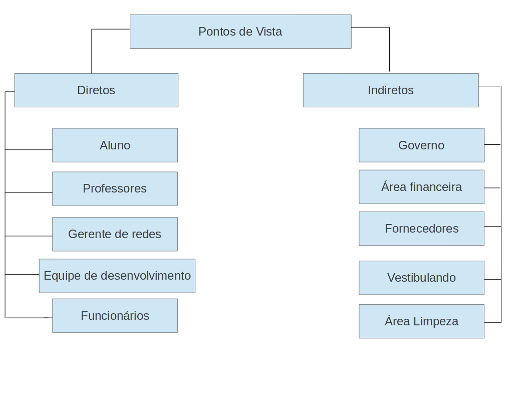
\includegraphics{hierarquia2}
	       \caption{Hierarquia de Pontos de Vista}
	       \label{figRotulo}
               \end{figure}
               
               
    
 \section{Modelagem do Sistema}
 
 É um modelo abstrato do sistema representando uma visão ou perspectiva.
 Para o sistema da empresa SOFT COMPANY são construídos modelos que explicam as características
 e o comportamento de todo o sistema na base de software.
 
   \begin{figure}[H]
	      \centering
	       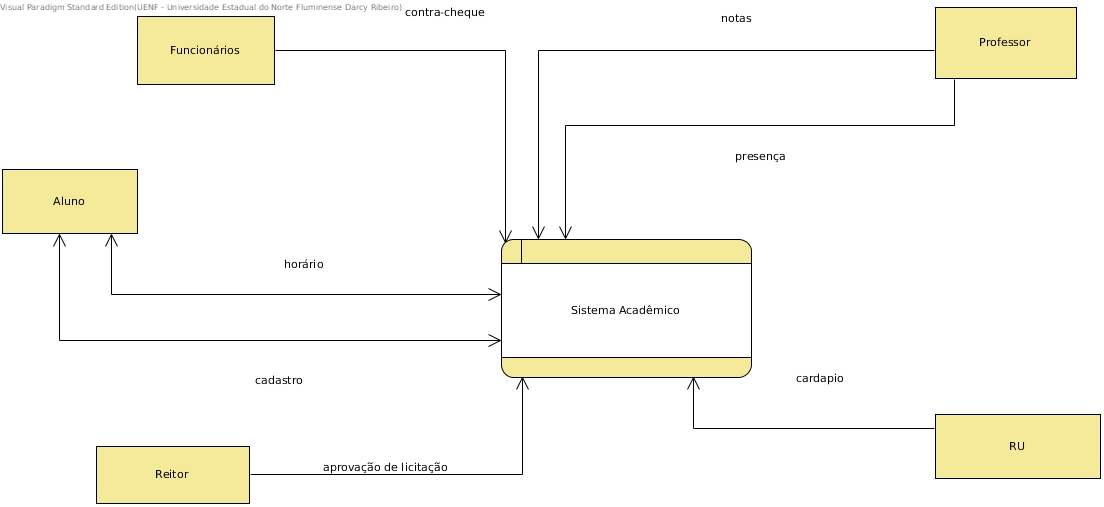
\includegraphics{diagrama1.jpg}
	       \caption{Modelo do sistema}
	       \label{figRotulo}
               \end{figure}
 